\documentclass[11pt]{report}
\clubpenalty=10000
\widowpenalty=10000

% input packages that I call bc they are in the template and I might want them.
\usepackage{amsmath}
\usepackage{amsfonts}
\usepackage{amssymb}
\usepackage{wasysym}
\usepackage{graphicx}
\usepackage{pslatex}
\usepackage{lscape}
\usepackage[T1]{fontenc}
\usepackage[latin1]{inputenc}
\usepackage{longtable}
 \setlength{\LTcapwidth}{5.5 in}
\usepackage{chapterbib}
\usepackage{fancyhdr} % for better header layout
\usepackage{eucal}
\usepackage[english]{babel}
\usepackage[usenames, dvipsnames]{color}
\usepackage[perpage]{footmisc}
\usepackage[round, sort, numbers, authoryear]{natbib}
%\usepackage{multicol} % for pages with multiple text columns, e.g. References
\setlength{\columnsep}{20pt} % space between columns; default 10pt quite narrow
\usepackage[nottoc]{tocbibind} % correct page numbers for bib in TOC, nottoc suppresses an entry for TOC itself
\usepackage{geometry}
\usepackage{setspace}
\usepackage{url}
\usepackage{lastpage}

% It is handy to define new commands for text that occurs frequently (see Discussion)
\newcommand{\MT}{^{\mathrm{MT}}}
\newcommand{\ga}{\gtrsim}
\newcommand{\Lpot}{(L+1)^2}
\newcommand{\WS}{^{\mathrm{WS}}}

%--Format the section headers

% FJS Changed this... I didn't like the numbering or the
% indentation... so I introduced a fake chapter Main Text. 
\setcounter{secnumdepth}{0}
\setcounter{tocdepth}{5}

%--set the page formatting--
\geometry{hmargin={1.6in,1.1in},vmargin={1.5in,1.2in}}
\doublespacing

%***********************************************************************************************************************************************************************************************************************************************************************************************************************************************************************

\begin{document}
%--front matter needs roman pagination--
\pagenumbering{roman}

%--Title Page--
\thispagestyle{empty}
  \begin{center}
    \textsc{\LARGE Spatial Localization of Greenland Mass Wasting Using a 2-D Wavelet Decomposition of GRACE Data and Comparison to Physical Drivers of Ice Loss} 
  \end{center}
  \vspace{.6in}
  \begin{center}
    Benjamin Getraer 
  \end{center}
  \vspace{.6in}
  \begin{center}
    \textsc{Senior Thesis Draft \\ 
    Presented to the Faculty \\
    of Princeton University \\
    in Candidacy for the Degree \\
    of Bachelor of Arts}
  \end{center}
  \vspace{.3in}
  \begin{center}
    \textsc{Recommended for Acceptance \\
    by the Department of \\
    Geosciences \\}
    Adviser: Laure Resplandy \\
    Second Reader: Frederik J.~Simons \\
  \end{center}
  \vspace{.3in}
  \begin{center}
\today
  \end{center}
  
  \clearpage

%--Copyright Page--
\thispagestyle{empty}
\vspace*{3in}
\begin{center}
\emph{This paper represents my own work in accordance with University regulations,} \\
Benjamin Getraer %%Sign here
\end{center}
\clearpage

%--Abstract--  
\addcontentsline{toc}{chapter}{Abstract}
\begin{center}
\Large \textbf{Abstract}
\end{center}
 % Senior thesis or Junior Project Abstract -----------------------------------------------------

% The premise for this paper is that there are significant unpredicted melt anomalies within the signal of the Greenland ice sheet seen in the GRACE timeseries. I believe that the global  spherical harmonic basis in which the GRACE data are released bias local Greenland signal with respect to other global gravitational anomalies, and obscure significant spatial information about the location and scale of sub-seasonal melt events. By transforming the GRACE time-series into bases which have concentrated support over Greenland we can gain a more accurate and informative understanding of where large scale mass-wasting events are occurring on the ice sheet, which in turn can help to confirm and inform our developing understanding of ice sheet -- atmosphere interactions.

Melting ice from the Greenland Ice-Sheet has accounted for an increasing percentage---now estimated at $25\%$---of rising global mean sea-level since the early 1990s. As recently as 2016, gravimetric and altimetric studies of Greenland melting rates found increasing rates of ice loss, which have not been borne out in GRACE gravimetric observations over the last few years (2015--2017). I investigate the correlations of atmospheric variables from MERRA-2 climate model reanalysis to show the ways in which temperature over the Greenland Ice Sheet has changed over the MERRA-2 (1980--) and GRACE (2003--2017) records. Our results not only confirm that temporal and spatial changes in GRACE derived mass loss are coincident with changes in near surface temperature, but demonstrate some of the limitations in GRACE spatial resolution, and contextualize recent variability in ice loss within the variability and long term trend of Greenland temperature. As Greenland Ice Sheet melting continues to be more unpredictable than early GRACE studies predicted, context is extremely important in both interpreting and communicating trends in ice loss. \\[3em]

\textbf{Key Points:}
\begin{enumerate}
	\item I focus on inter-annual variability of the Greenland ice loss trend.
	\item I contextualize recent variation in melt and temperature through analysis of 1980--2017 MERRA-2 climate reanalysis data. 
%	\item We find unexpected periodic structure of $3$--$7$ years in the Greenland ice loss trend.
%	\item .

\end{enumerate}
 \clearpage

%--Acknowledgements--  
\addcontentsline{toc}{chapter}{Acknowledgements}
\begin{center}
\Large \textbf{Acknowledgements}
\end{center}
% Senior thesis or Junior Project Acknowledgements  -----------------------------------------------------

Thank you to my thesis adviser Prof.~Laure Resplandy who has helped me understand and think through atmospheric processes and the direction this project has taken this year.
Thank you to my Junior Paper adviser Prof.~Frederik J.~Simons who helped me with
the conceptualization, direction, and revision of earlier portions of this project. Thank you to the second reader of my Fall Junior Paper, Prof.~Jessica Irving for feedback, suggestions, and encouragement. Thanks to Dr.~Amanda
Irwin Wilkins and ``The Hare'' writing workshop group for discussing
and editing various figures and drafts of my Junior Papers. Thank you to Prof.~Adam C.~Maloof who taught me \LaTeX, and to Dr.~Chris Harig for providing some of the data files. Thank you to Prof.~Gabriel Vecchi for insight into atmospheric and oceanic processes. Thank you to Jean Getraer, Andrew Getraer, Jonathan Feld, Rae Perez, and Zach Smart for proof-reading various Junior Paper drafts.  Lastly, thank you to the numerous professors and graduate and undergraduate students in the Princeton Department of Geosciences for feedback, encouragement, and constructive criticism on various presentations of preliminary results. A big thanks especially to all of the people who asked me, ``What is your independent work about?'' and then patiently listened while I struggled to articulate this project in a way that made any sense.

\clearpage

%--Table of Contents--  
\thispagestyle{empty}
\tableofcontents
\clearpage

\listoffigures
\listoftables
\clearpage

%--Set up fancy header-- 
\fancyhead{}
\fancyfoot{}
\pagestyle{fancyplain}
\rhead{\fancyplain{\thepage}{\noindent \textsc{\rightmark} \hfill \thepage~of~\pageref{LastPage}}}
\rfoot{\hrule \today \hfill Benjamin Getraer}
\pagenumbering{arabic}

%--Reset the page numbers and set them to arabic-- 
{\newpage\renewcommand{\thepage}{\arabic{page}}\setcounter{page}{1}}

%--Have sections but use chapter counters
\addcontentsline{toc}{chapter}{Main Text}

\section{Introduction \label{sec:introduction}}

Average global surface temperature is rising at an increasing rate --- approximately $0.09\degree$~C per decade since 1880, and approximately $0.26\degree$~C per decade since 1979 \cite[][]{ipcc2013_atmosphere}
--- and has contributed to significant melting of the
Greenland ice sheet, with recent ice loss approximated at $-244$~Gt per
year \cite[][]{Harig+2015a,Harig+2016}. The Greenland Ice Sheet covers just over 1\% of
Earth's surface, and, if completely melted, would raise sea level by over $7$~m
\cite[][]{ipcc2013_cryosphere}.
Massive loss of ice has
significant repercussions for human civilization, bringing with it a rising sea
level at about $1$--$2$~mm per year at the end of 2010
\cite[][]{ipcc2013_sealevel}.  Our broad goal is to understand deviations from modeled rates of Greenland ice melt in order to better understand, predict, and
communicate the changing conditions of the planet.


\begin{figure}[h!]
\centering
\makebox[\textwidth][c]{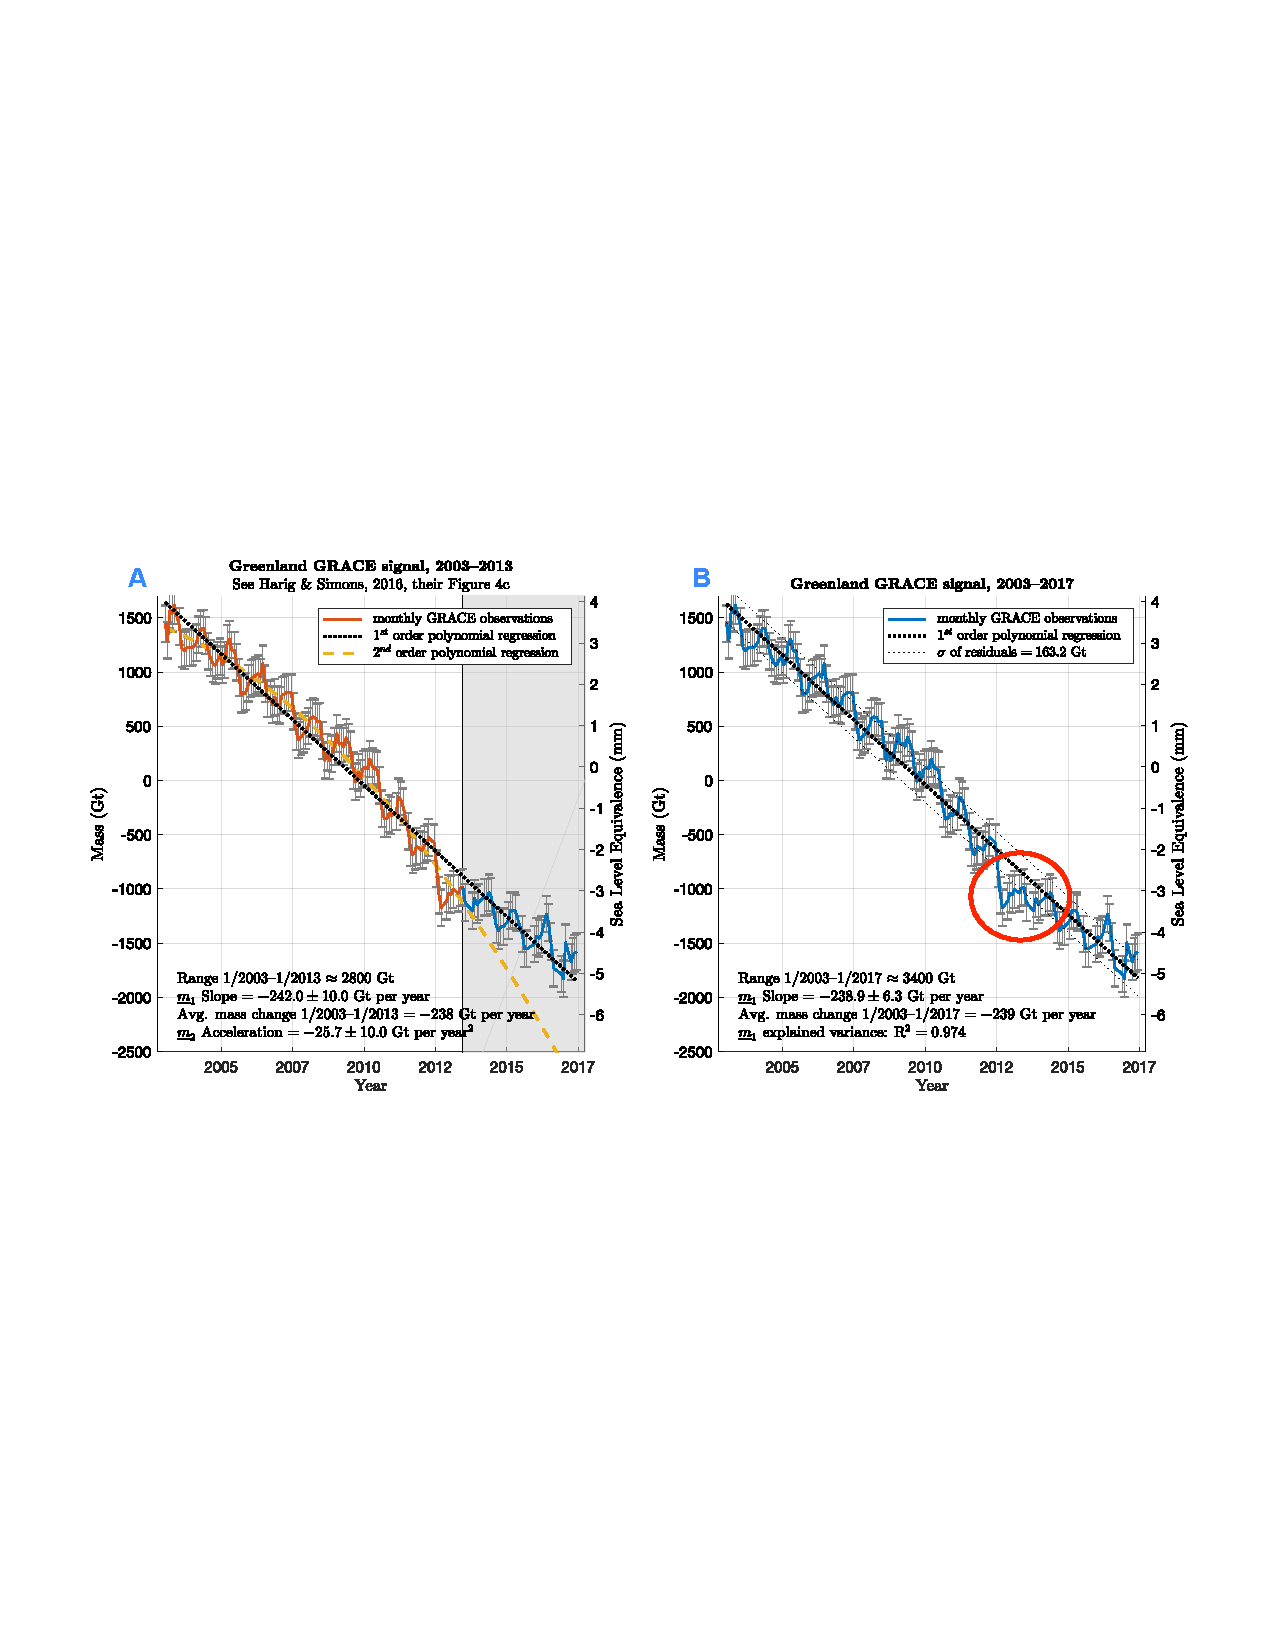
\includegraphics[height=0.37\textheight]
{Figures/HarigGetraerTrend.pdf}}
\caption[Greenland Mass Trend: 2003--2017]{Total mass changes for Greenland over the complete GRACE record using equivalent methods to \cite{Harig+2016}. Shown in \textbf{A} are the $\underline{m}_1$ (linear) and $\underline{m}_2$ (quadratic) models for 01/2003--06/2013, comparable to previous estimates of the mass trend \citep{Harig+2016}. Note the significant departure of the extrapolated $\underline{m}_2$ model from the continuing signal. Shown in \textbf{B} is the $\underline{m}_1$ linear model for 01/2003--06/2017 with the standard of deviation of its residuals. Note that the $\underline{m}_1$ model does not significantly change after including the entire GRACE record. Error bars represent $2\sigma$ based on the combined variance of modeled Slepian coefficients $f_{\alpha}$ (see \cite{Harig+2016}, as well as \cite{getraerFall,getraerSpring}). This figure appeared in \cite{getraerFall,getraerSpring}, here with minor updates.} \label{fig:Getraer}
\end{figure}

Ice mass of the Greenland Ice Sheet has been calculated using
gravimetric data from NASA's Gravity
Recovery and Climate Experiment (GRACE), as well as satellite and airplane based
altimetry, finding decreasing rates in the ice mass signal over the last
decade \cite[][]{khan2015,Harig+2016}. Rates of ice loss increase by a
combination of greater discharge from calving glacier termini at the edges of
the ice-sheet and decreased surface mass-balance, the difference between
seasonal snow accumulation and melting \cite[][]{khan2015,enderlin2014}.
Significant inter-annual variability and asynchronicity has been observed in
the discharge rates of the Greenland Ice Sheet's major drainage basins, while
surface mass-balance is comparatively more predictable
\cite[][]{mcmillan2016,enderlin2014}. Both contributions to ice loss accelerated between 2000--2012, combining for a total acceleration of ice mass
estimated around $-30$~Gt per year$^2$ over all of Greenland
\cite[][]{velicogna2009,enderlin2014}.

\begin{figure}[h!]
\centering
\makebox[\textwidth][c]{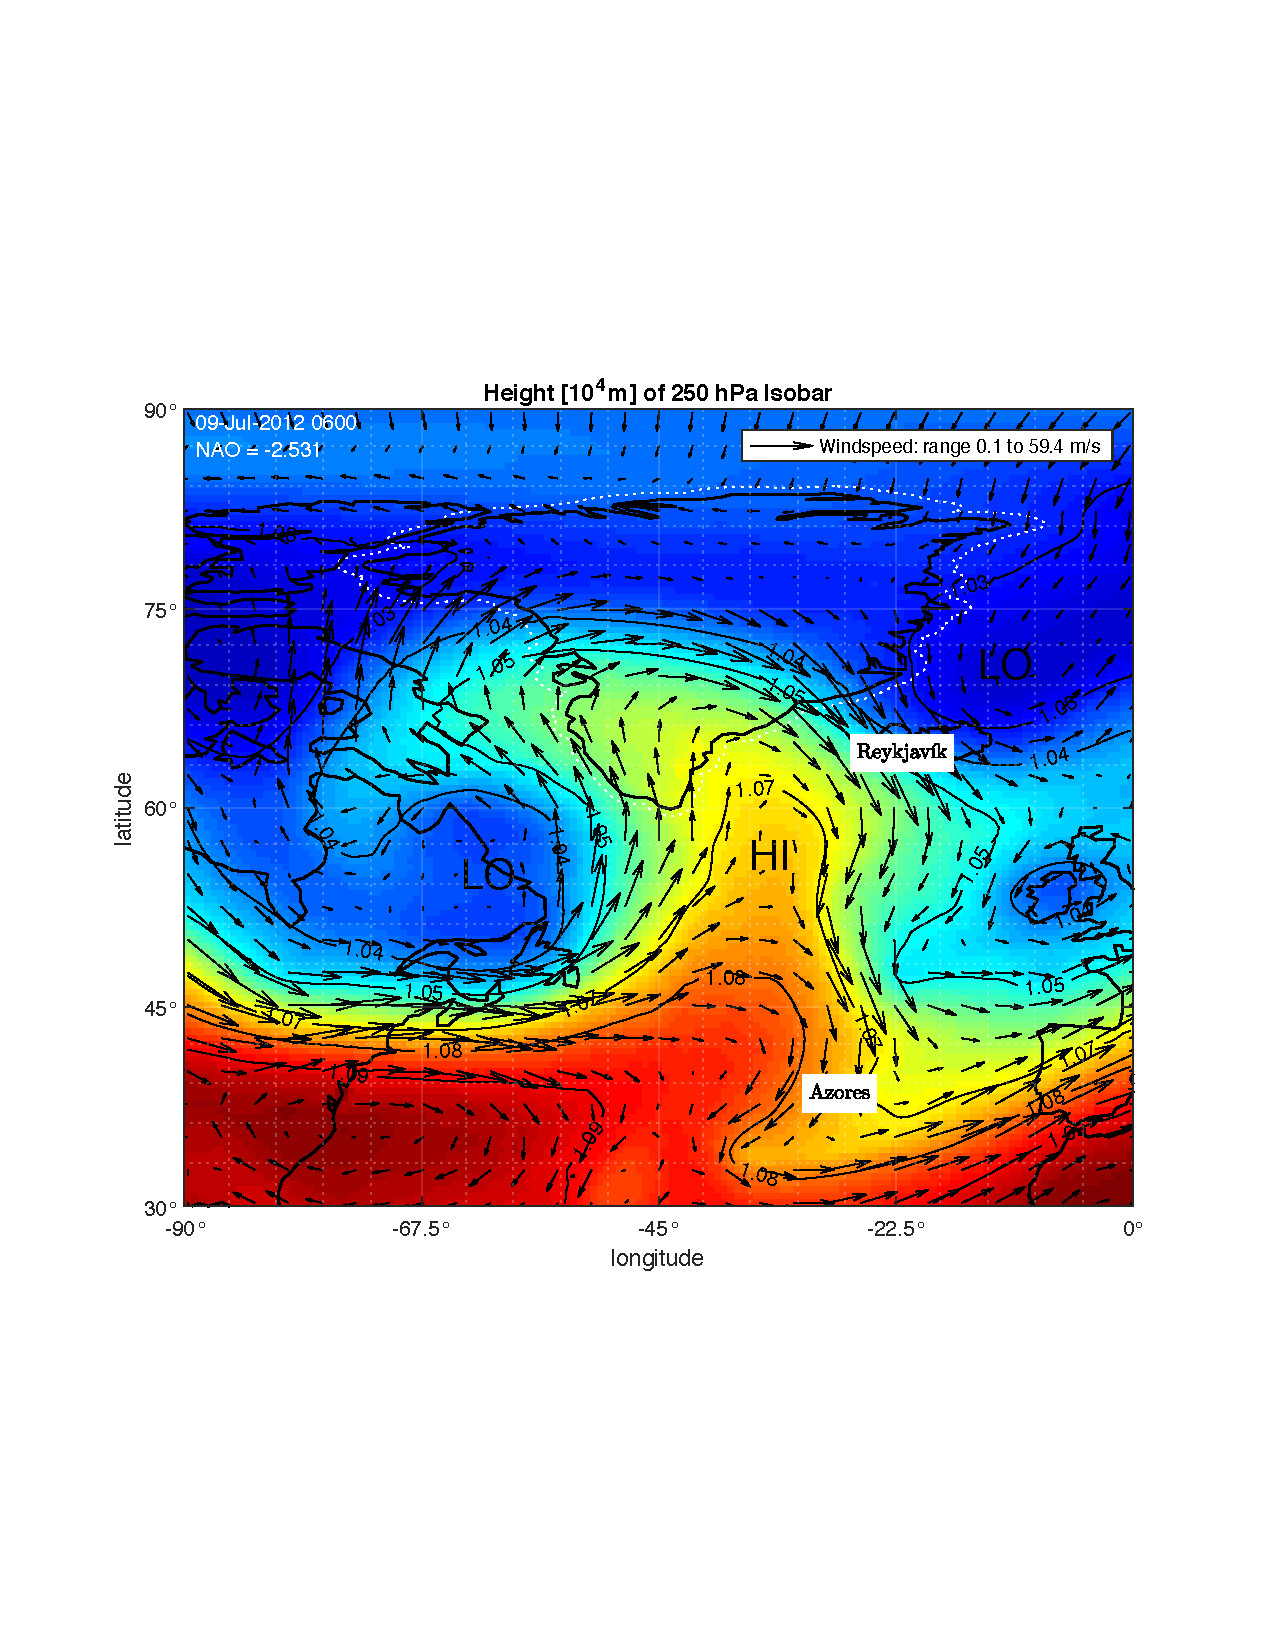
\includegraphics[height=0.5\textheight]
{Figures/jetstream.pdf}}
\caption[Atmospheric Circulation Around Greenland]{Example of atmospheric conditions at the $250$~hPa isobar over the North Atlantic preceding record Greenland Ice Sheet surface melt, 07/09/2012 (from MERRA-2 reanalyzed data). Isobar height contours are labeled in $10^4$~m, and wind vectors are shown by arrows. Note the location of the northern polar jet stream, dividing the low and high isobar heights around the $1.05\times 10^{4}$~m contour. The temporary North Atlantic Rossby wave is labeled as the ``HI'' pressure anti-cyclone moving north towards southern Greenland, with a complementary ``LO'' pressure cyclone centered over Labrador. Note that the jet stream is deflected through the Labrador Sea and Baffin Bay, along the West Coast of Greenland. As a result of these conditions, the ``LO'' pressure over Reykjav\'ik is pushed north, and the pressure difference between Reykjav\'ik  and Azores is lowered, resulting in an negative NAO index (top left).} \label{fig:jetstream}
\end{figure}

A study by \cite{Harig+2016} modeling the mass of the Greenland Ice Sheet
using GRACE data products showed deviations from the long-term quadratic
trend, starting with a high level of melt in the summer of 2012, and followed by two
summers of little melting in 2013 and 2014 \cite[see
Figure~\ref{fig:Getraer} A, comparable to][their
Figure~4]{Harig+2016}. Our analysis of the complete GRACE data set (2002--2017) using identical methods showed a linear,
not accelerating, trend of ice loss for the Greenland Ice Sheet, constraining the observed unexpected deviations to an unusually large melt summer of 2012 followed by a summer of unusually little melt in 2013 (see
Figure~\ref{fig:Getraer} B). 


The anomalous seasons of 2012--2013 have received attention in recent literature by studies attempting to understand how surface mass balance processes could produce such inter-annual variability. Explanations and correlations have been found relationships with climate indices such as the phase of the North Atlantic Oscillation (NAO) \cite[][]{mcmillan2016,bevis2018,getraerFall}, transient atmospheric transport of warm air and water vapor in so-called "atmospheric rivers" \citep{mattingly2018}, and non-radiative energy flux caused by short-term cloud cover \citep{solomon2017}. 

\begin{wrapfigure}{r}{0.5\textwidth} 
\vspace{-20pt}
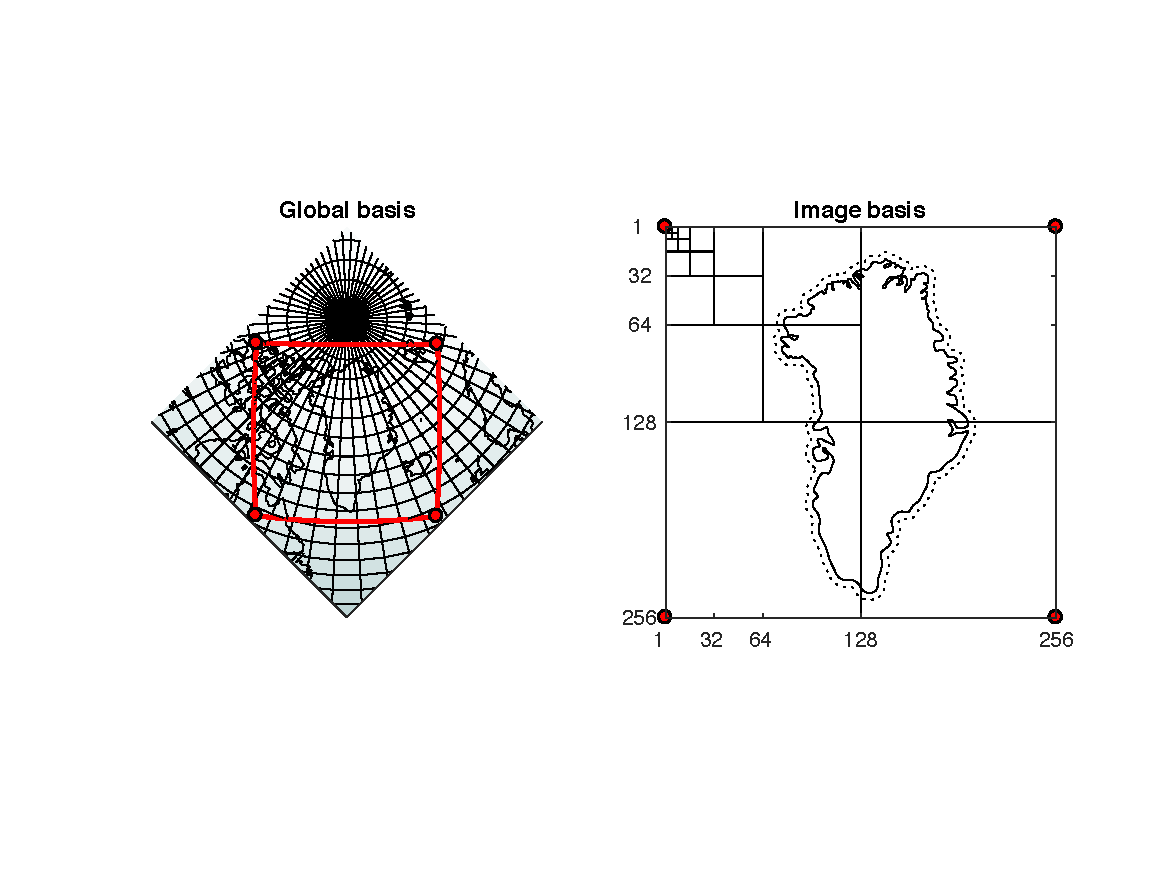
\includegraphics[width=1.1\linewidth]{Figures/thegrid.pdf}
\caption[The Discrete Grid Around Greenland]{A grid is defined in the global basis on a face of the Cubed Sphere centered on Greenland, upon which the gravitational anomaly is evaluated from the GRACE spherical harmonic solutions. In the image basis the grid is cartesian with length $256$. Grid lines in the image basis represent the diminishing spatial support of wavelets of different levels, from $\zeta=8$ (the entire image) to $\zeta=1$ (a unit grid cell). Note that in reality, each wavelet level has coverage over the entire image. The dotted line around Greenland is a coastal buffer of $0.5^{\circ}$ as in \cite{Harig+2016}. This Figure appeared in my Spring JP.} \label{fig:thegrid}
%\vspace{-50pt}
\end{wrapfigure}

The atmospheric circulation affecting the Greenland Ice Sheet is broadly controlled by the position of the polar jet stream in the northern hemisphere \cite[][]{hanna2013,mattingly2018}. Specifically, strong summer melt events often occur with a negative NAO index and high pressure ``blocking'' over southern Greenland, advecting warm moist air into the Arctic along the west coast of Greenland \cite[][]{hanna2013,mattingly2018,mcmillan2016,bevis2018,getraerFall}. The NAO index broadly represents the difference in atmospheric pressure between the typically cold, low-pressure Arctic air near Reykjav\'ik, Iceland, and the typically warm, high-pressure air near Azores, Portugal, divided by the location of the polar jet stream (see Figure~\ref{fig:jetstream}). When the Azores high-pressure system pushes the jet stream northward, the pressure difference across the North Atlantic is weaker, producing a negative NAO index (Figure~\ref{fig:jetstream}). This temporary high-pressure excursion into the arctic is known as a Rossby wave and is accompanied by complementary low-pressure cyclones which develop on either side of the high-pressure block, the combined flow from which advects warm air into the Arctic until the Rossby wave ``breaks'' and the jet stream return to its typical location. These atmospheric conditions are illustrated in Figure~\ref{fig:jetstream}, illustrating the Greenland blocking event in July 2012, immediately preceding record surface melting on the Greenland Ice Sheet on 07/11/2012 \cite[][]{hanna2013,mattingly2018}.





The general conclusions drawn by these studies point to common atmospheric processes of uncommon duration or intensity. 





\subsection{Previous Results \label{sec:prevresults}}

\begin{wrapfigure}{r}{0.5\textwidth} 
\vspace{-50pt}
%\centering
%\makebox[\textwidth][c]{
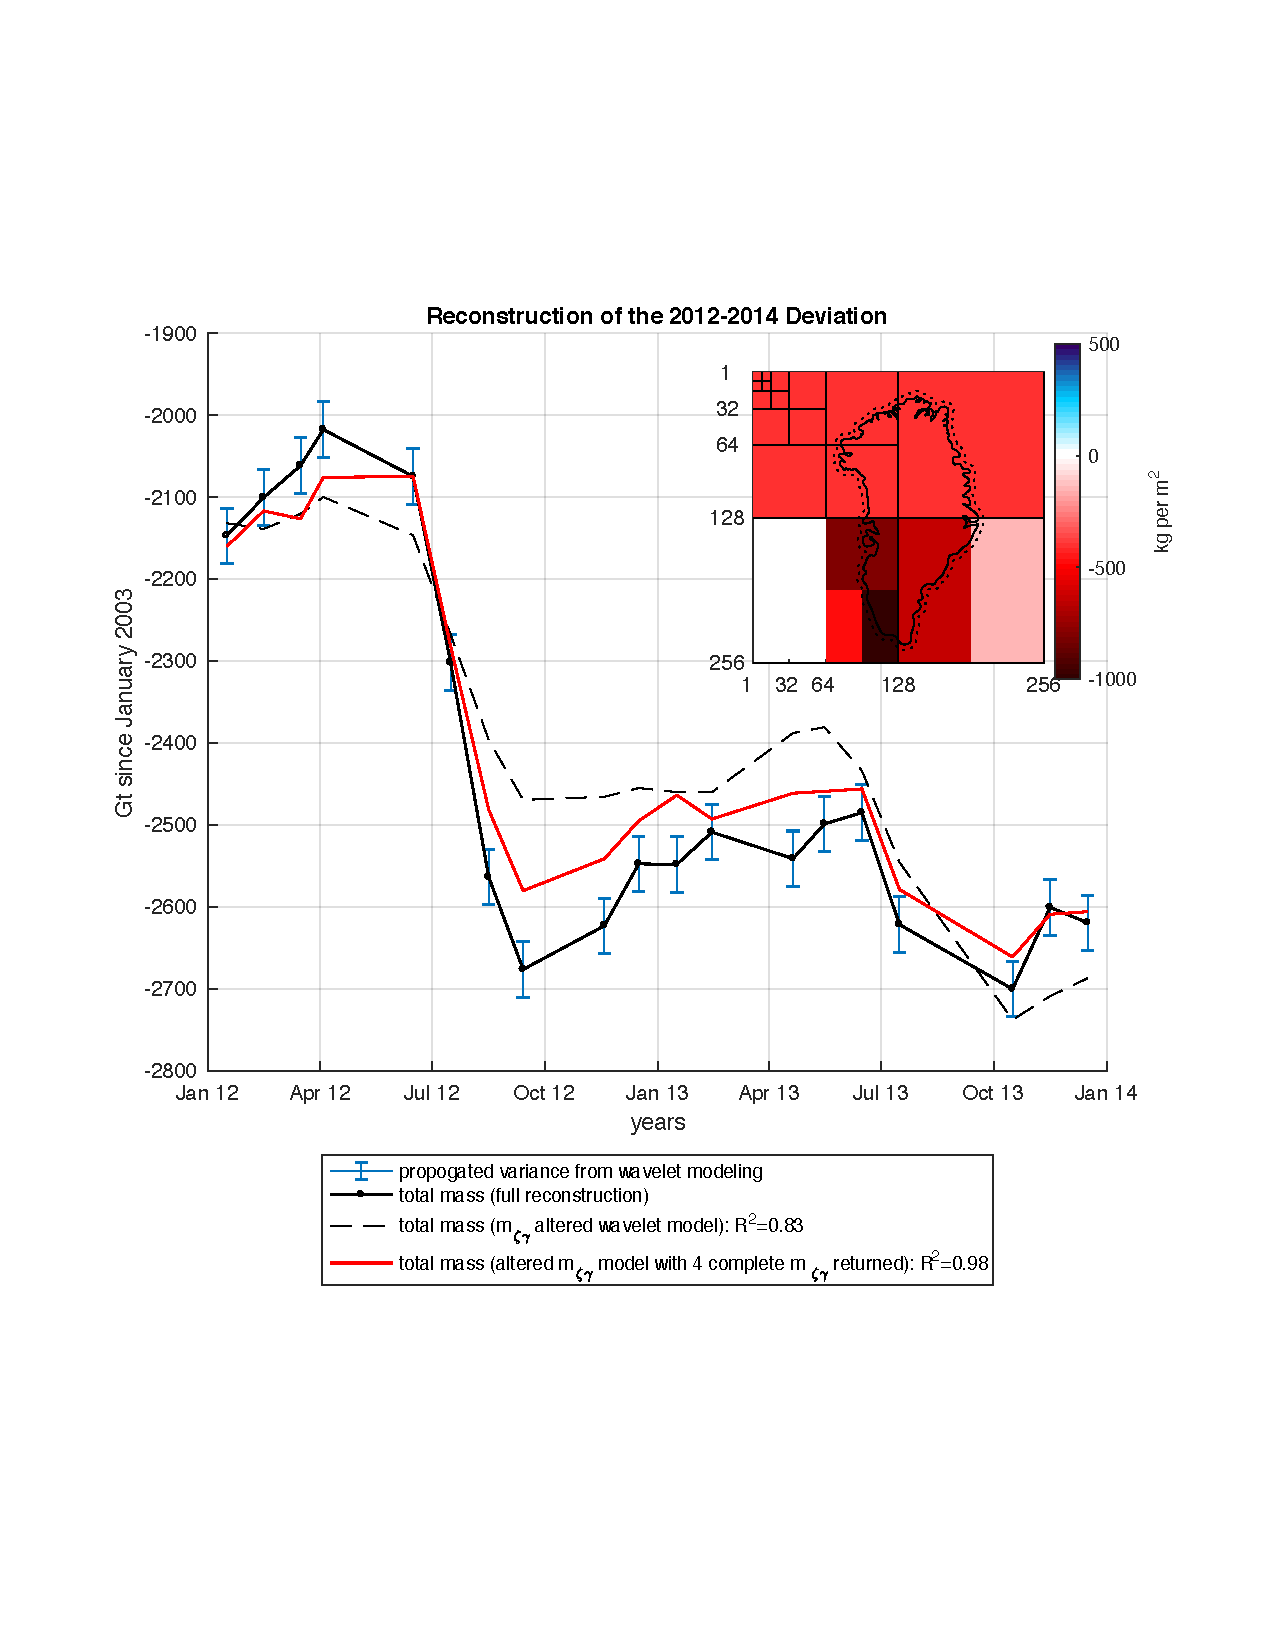
\includegraphics[width=\linewidth]{Figures/deviant.pdf}
%}
\caption[Location of the 2012--2014 Deviation]{The 2012--2014 deviation in Greenland mass and the total from the reconstructed modeled wavelet coefficients. By adding in the real values of only four wavelet coefficients back into the modeled wavelet reconstruction we improve the variance explanation by $15\%$. These wavelets are shown inset, weighted by their values in September 2012, the extreme of the deviation, and are concentrated in southwestern Greenland. ``m$_{\zeta\gamma}$'' refers to a wavelet basis function ``m'' of index $\gamma$ in level $\zeta$. This Figure appeared in my Spring JP.
\label{fig:deviant}}
\end{wrapfigure}

In my Spring 2018 JP, I explored the use of a 2-D wavelet basis to represent the GRACE gravimetric data over Greenland such that meaningfully contributing basis functions also contained information about spatial structure (see
Figure~\ref{fig:thegrid}). 

I developed a procedure for choosing the most important wavelet basis functions in order to extract the true fluctuation of the signal from the over-determined image calculated from the typical GRACE spherical harmonic basis. I then tested which wavelet basis function best captured the 2012--2013 deviation from the expected signal, finding the deviations to be concentrated in southwestern Greenland (see
Figure~\ref{fig:deviant}). 






\section{Next steps}

\begin{enumerate}
\item get updated GRACE RL06 data
\item quantitative image to image comparison of moisture transport and mass loss
\item calculate mass loss on a sub basin spatial level across Greenland and compare to other estimates
\item test wavelet results using different bases
\end{enumerate}

The NAO index is unitless, and represents the relative magnitude of the 500mb pressure difference between Azores and Reykjav\'ik compared to the 1950--2000 monthly mean.

%http://www.cpc.ncep.noaa.gov/products/precip/CWlink/pna/nao_loading.html

% APPENDIX A --- DATA SOURCES
\newpage 
\appendix

\section{Appendix A: Data and code sources \label{app:a}}

\textit{RL05 spherical harmonic coefficients for the time-variant geopotential field from the Center for Space Research data processing center at The University of Texas at Austin are available at:} \\
\indent \url{ftp://podaac.jpl.nasa.gov/allData/grace/L2/CSR/RL05}\\

\noindent\textit{Coefficients describing Earth's center of mass \cite[spherical harmonic degree~1, from][]{swenson2008} are available at:} \\
\indent\url{ftp://podaac-ftp.jpl.nasa.gov/GeodeticsGravity/tellus/L2/degree_1/}\\

\noindent\textit{Coefficients describing Earth's oblateness \cite[spherical harmonic degree~2, order~0, from][]{cheng2013} are available at:} \\
\indent \url{ftp://ftp.csr.utexas.edu/pub/slr/degree_2/}\\

\noindent\textit{Index values for the North Atlantic Oscillation are calculated by the National Weather Service Climate Prediction Center \cite[see][]{cpcNAO}, with normalized monthly average values since January 1950 available at:} \\
\indent \url{ftp://ftp.cpc.ncep.noaa.gov/wd52dg/data/indices/nao\_index.tim}\\
\indent\textit{Normalized daily values since January 1950 are available at:} \\
\indent \url{ftp://ftp.cpc.ncep.noaa.gov/cwlinks/norm.daily.nao.index.b500101.current.ascii}\\


\noindent\textit{MERRA-2 atmospheric reanalysis data are calculated by the NASA Global Modeling and Assimilation Office (GMAO) as part of the activities of NASA's Science Mission Directorate, and are archived and distributed by the Goddard Earth Sciences Data and Information Services Center (GES-DISC). All data was accessed between September 2018 and April 2019.} \\ 
\indent \textit{A graphical user interface for generating data download links for specific subsets of variables, space, and time is available at:} \url{https://disc.gsfc.nasa.gov}\\
\indent \textit{Data used in this study can be directly accessed at the following addresses:} \\
\indent \url{https://goldsmr4.gesdisc.eosdis.nasa.gov/data/MERRA2_MONTHLY/M2SMNXSLV.5.12.4/}\\
\indent \url{https://goldsmr4.gesdisc.eosdis.nasa.gov/data/MERRA2/M2T1NXSLV.5.12.4/}\\
\indent \url{https://goldsmr4.gesdisc.eosdis.nasa.gov/data/MERRA2/M2T1NXRAD.5.12.4/}\\


\noindent\textit{Northern Hemisphere Land-Ocean Temperature Index anomalies from NASA's Goddard Institute for Space Studies Surface Temperature Analysis \cite[GISTEMP v3, see][]{hansen2010} were accessed in March 2019 and are available at:} \\ 
\indent \url{https://data.giss.nasa.gov/gistemp/tabledata_v3/NH.Ts+dSST.csv}\\



\noindent\textit{MATLAB code for the expansion and manipulation of spherical harmonic
eigenfunctions into Slepian bases and manipulation of GRACE files is borrowed and adapted from:} \\
\indent \url{https://github.com/csdms-contrib/}\\

\noindent\textit{MATLAB code developed for this project, including functions for executing the wavelet analysis and scripts for generating figures, can be accessed at:} \\
\indent \url{https://github.com/bgetraer/slepian_bgetraer/}\\




%\noindent\textit{Outline coordinates for the Greenland ice scheet drainage basins from \cite{zwally} available at:}\\
%\indent \url{http://icesat4.gsfc.nasa.gov/cryo_data/ant_grn_drainage_systems.php}\\


%--References
\small
\renewcommand{\bibsep}{0em}

\renewcommand{\bibname}{References}
\bibliographystyle{/Users/benjamingetraer/Documents/IndependentWork/LatexFiles/gji.bst}
\bibliography{/Users/benjamingetraer/Documents/IndependentWork/LatexFiles/bgetraerBib.bib}




\end{document}